\section{RV12 Execution Pipeline}

Lorem ipsum dolor sit amet, consectetur adipiscing elit, sed do eiusmod tempor incididunt ut labore et dolore magna aliqua. Vitae tempus quam pellentesque nec nam aliquam sem. Quis eleifend quam adipiscing vitae proin sagittis nisl. Amet consectetur adipiscing elit pellentesque. Augue neque gravida in fermentum et sollicitudin ac orci. Elementum sagittis vitae et leo duis. A pellentesque sit amet porttitor eget dolor morbi. Magna fermentum iaculis eu non diam phasellus vestibulum lorem sed. Commodo nulla facilisi nullam vehicula ipsum a arcu cursus vitae. Netus et malesuada fames ac turpis egestas integer. Magna ac placerat vestibulum lectus mauris ultrices eros in cursus. Commodo elit at imperdiet dui accumsan. \todo{add introduction to pipeline section}

\begin{figure}[h]
  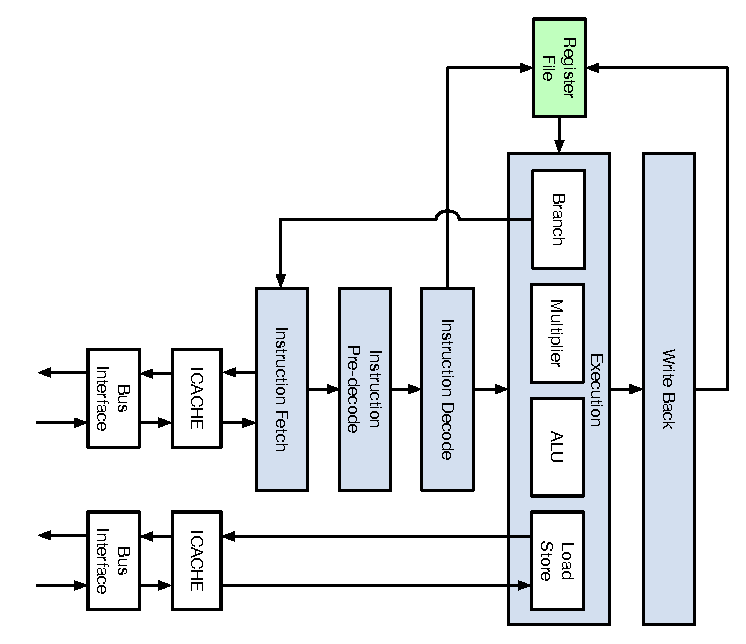
\includegraphics{Pipeline-Overview}
  \caption{RV12 Execution Pipeline}
\end{figure}

\pagebreak

\subsection{Instruction Fetch (IF)}\label{instruction-fetch-if}

\begin{figure}[h]
  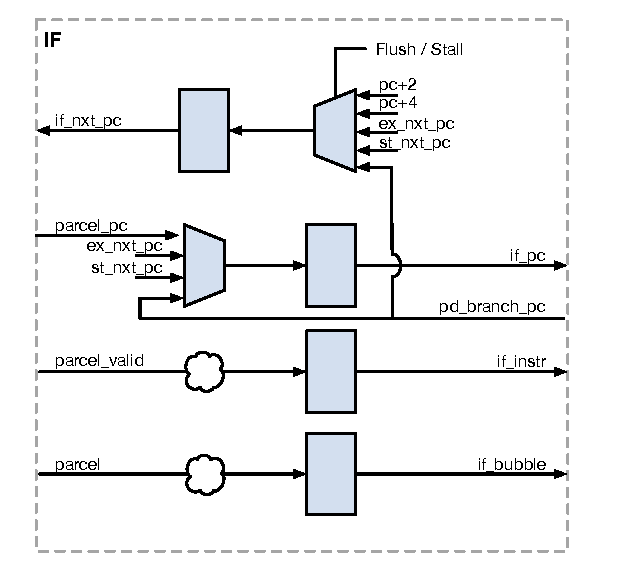
\includegraphics{Pipeline-IF.eps}
  \caption{Instruction Fetch Stage Implementation}
\end{figure}

The Instruction Fetch unit loads a new parcel from the program memory. A
parcel is a code field that contains one or more instructions. The
address of the parcel to load is held by the Program Counter (PC). The
Program Counter is either 32 or 64bits wide, depending on the XLEN
parameter. The Program Counter is updated whenever the Instruction
Pipeline is not stalled.

The Instruction Fetch unit translates 16-bit compressed instructions to
base 32bit RISC-V instructions and then processes Program Counter
modifying instructions. Jump-And-Link and Branch instructions modify the
Program Counter in the Instruction Fetch unit. This avoids waiting for
the Execute stage to trigger the update and removes the demand for
pipeline flushes. The destination address for branches is predicted
based on the data provided by the optional Branch Prediction unit or
determined statically based on the offset.

In case the pipeline must be flushed the Program Counter is restarted
from the given address.

\pagebreak

\subsection{Pre-Decode (PD)}\label{pre-decode-pd}

Lorem ipsum dolor sit amet, consectetur adipiscing elit, sed do eiusmod tempor incididunt ut labore et dolore magna aliqua. Vitae tempus quam pellentesque nec nam aliquam sem. Quis eleifend quam adipiscing vitae proin sagittis nisl. Amet consectetur adipiscing elit pellentesque. Augue neque gravida in fermentum et sollicitudin ac orci. Elementum sagittis vitae et leo duis. A pellentesque sit amet porttitor eget dolor morbi. Magna fermentum iaculis eu non diam phasellus vestibulum lorem sed. Commodo nulla facilisi nullam vehicula ipsum a arcu cursus vitae. Netus et malesuada fames ac turpis egestas integer. Magna ac placerat vestibulum lectus mauris ultrices eros in cursus. Commodo elit at imperdiet dui accumsan. \todo{Add description}

\begin{figure}[th]
  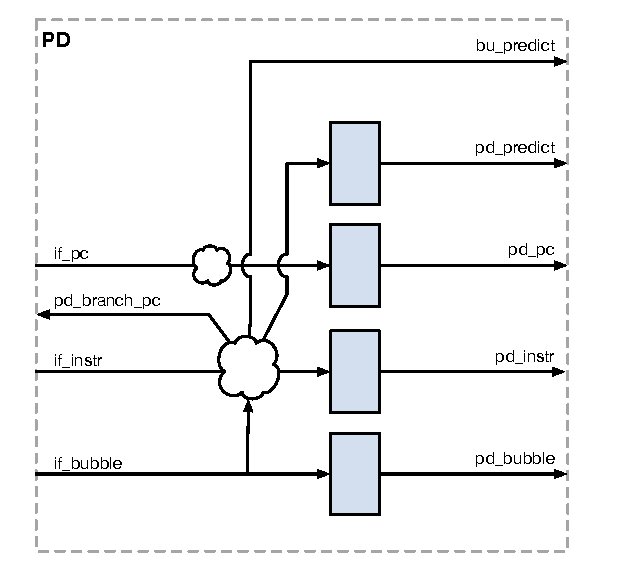
\includegraphics{Pipeline-PD.eps}
  \caption{Instruction Pre-Decode Stage}
\end{figure}

\pagebreak

\subsection{Instruction Decode (ID)}\label{instruction-decode-id-1}

The Instruction Decode unit ensures the operands for the execution units
are available. It reads the Register File values, calculates immediate
values, and sets bypasses.

The Instruction Decode unit stalls the pipeline when an operand value is
not available. The RV12 only stalls when a value is loaded from data
memory and is used in the instruction immediately after the load.

\begin{figure}[h]
  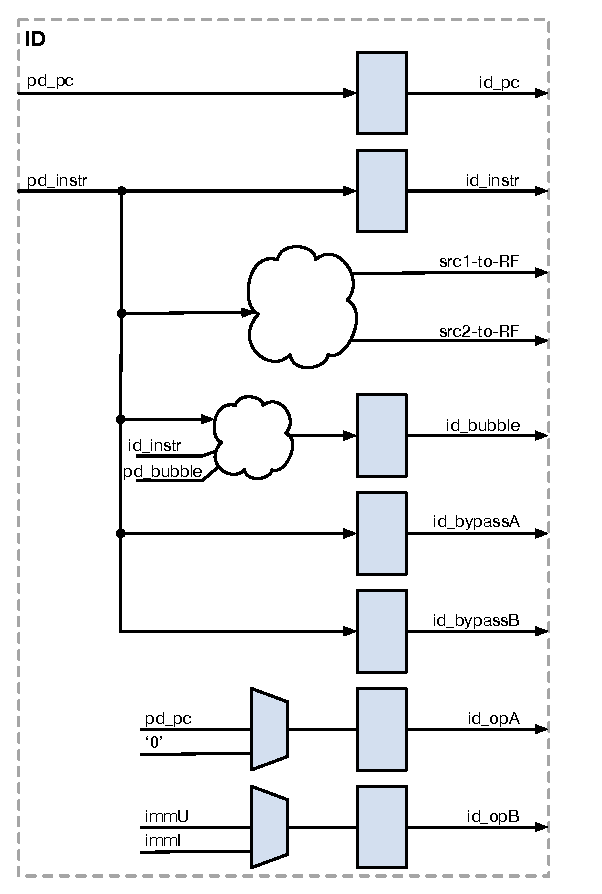
\includegraphics{Pipeline-ID.eps}
  \caption{Instruction Decode Stage Implementation}
\end{figure}

\pagebreak

\subsection{Execute (EX)}\label{execute-ex-1}

The Execute/Memory-Access stage performs the required operation on the
data provided by the decode stage. It performs logical or arithmetic
operations using the Arithmetic-Logical-Unit (ALU), calculates jump and
branch addresses, performs Read-Modify-Write accesses to the CSRs, and
starts memory accesses using the Memory Unit. Only one operation can be
executed per clock cycle.

\begin{figure}[h]
  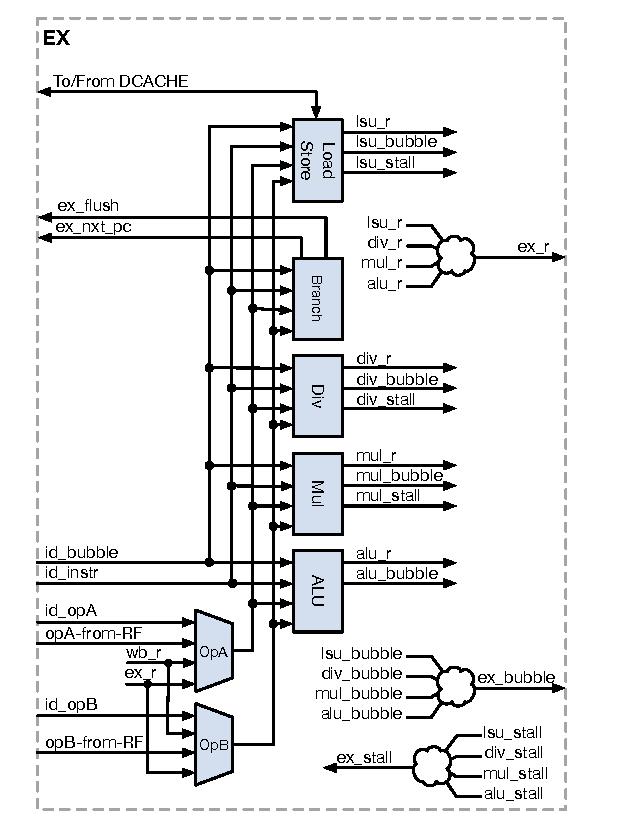
\includegraphics{Pipeline-EX.eps}
  \caption{Execute Stage Implementation}
\end{figure}

\pagebreak

\subsection{Write-Back (WB)}\label{write-back-wb-1}

The Memory/Write-Back stage completes a pending memory access and writes
the results from the ALU or the Memory Unit into the Register File.

\begin{figure}[h]
  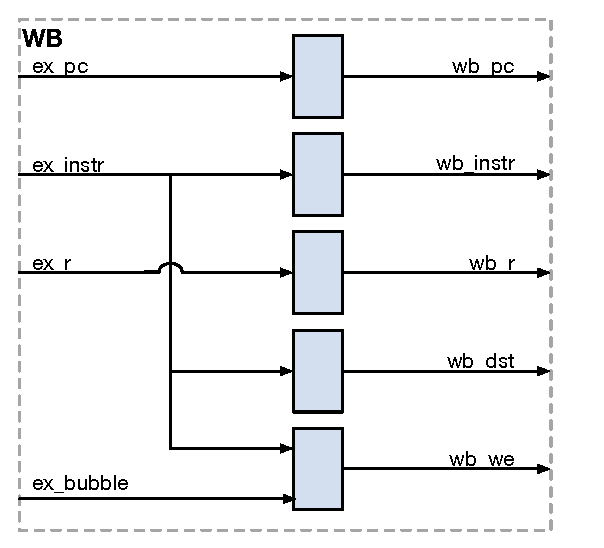
\includegraphics{Pipeline-WB.eps}
  \caption{Write-back Stage Implementation}
\end{figure}